\documentclass[a4paper, 12pt,oneside]{article}
%On peut changer "oneside" en "twoside" si on sait que le résultat sera recto-verso.
%Cela influence les marges (pas ici car elles sont identiques à droite et à gauche)

% pour l'inclusion de figures en eps,pdf,jpg,....
\usepackage{graphicx}
\usepackage{subcaption}

\usepackage{amssymb}

\usepackage{float}
\usepackage{caption}
\usepackage{multirow}



%Marges. Désactiver pour utiliser les valeurs LaTeX par défaut
%\usepackage[top=2.5cm, bottom=2cm, left=2cm, right=2cm, showframe]{geometry}
\usepackage[top=2.5cm, bottom=2cm, left=2cm, right=2cm]{geometry}
% quelques symboles mathematiques en plus
\usepackage{amsmath}

% le tout en langue francaise
%\usepackage[francais]{babel}

% on peut ecrire directement les charactères avec l'accent
\usepackage[T1]{fontenc}

% a utiliser sur Linux/Windows
%\usepackage[latin1]{inputenc}

% a utiliser avec UTF8
\usepackage[utf8]{inputenc}
%Très utiles pour les groupes mixtes mac/PC. Un fichier texte enregistré sous codage UTF-8 est lisible dans les deux environnement.
%Plus de problème de caractères accentués et spéciaux qui ne s'affichent pas

% a utiliser sur le Mac
%\usepackage[applemac]{inputenc}

% pour l'inclusion de liens dans le document (pdflatex)
\usepackage[colorlinks,bookmarks=false,linkcolor=black,urlcolor=blue, citecolor=black]{hyperref}

%Pour l'utilisation plus simple des unités et fractions
\usepackage{units}

%Pour utiliser du time new roman... Comenter pour utiliser du ComputerModern
%\usepackage{mathptmx}

%Pour du code non interprété
\usepackage{verbatim}
\usepackage{verbdef}% http://ctan.org/pkg/verbdef

%Pour changer la taille des titres de section et subsection. Ajoutez manuellement les autres styles si besoin.
\makeatletter
\renewcommand{\section}{\@startsection {section}{1}{\z@}%
             {-3.5ex \@plus -1ex \@minus -.2ex}%
             {2.3ex \@plus.2ex}%
             {\normalfont\normalsize\bfseries}}
\makeatother

\makeatletter
\renewcommand{\subsection}{\@startsection {subsection}{1}{\z@}%
             {-3.5ex \@plus -1ex \@minus -.2ex}%
             {2.3ex \@plus.2ex}%
             {\normalfont\normalsize\bfseries}}
\makeatother

%Début du document
\begin{document}


\begin{center}
\large\textbf{\sffamily Deterministic Chaos}\\%
\large\sffamily Group N$^\circ$1: Alexis Escarmelle, Nil Fajas\\%
\large\sffamily \today\qquad Francesco Ciccarello\\%
\end{center}

%			Introduction
\section{Introduction}
Quantum entanglement is one of the most striking and counterintuitive phenomena in quantum mechanics, challenging classical notions of locality and reality. First formally discussed by Schrödinger in 1935, entanglement describes a situation where the quantum state of a composite system cannot be factorized into independent states of its subsystems \cite{Schrodinger}. This phenomenon was at the heart of a famous debate initiated by Einstein, Podolsky, and Rosen (EPR) in their seminal paper, where they questioned whether quantum mechanics could be considered a complete theory \cite{EPR}. EPR formulated a thought experiment suggesting that quantum mechanics allows for nonlocal correlations between distant particles, leading them to argue in favor of hidden variables that would restore determinism to physical theory.

The implications of entanglement remained largely theoretical until the groundbreaking work of John Bell in 1964, who derived what are now known as Bell's inequalities \cite{Bell}. Bell demonstrated that if hidden-variable theories governed quantum mechanics, the correlations predicted by quantum theory should obey certain mathematical constraints. However, quantum mechanics predicts violations of these inequalities, implying that no local hidden-variable theory can fully describe quantum reality.

The definitive experimental confirmation of quantum entanglement came in 1982 with the pioneering work of Alain Aspect and his collaborators \cite{Alain Aspect}. Their experiment involved measuring polarization correlations in entangled photon pairs, implementing fast-switching detection schemes to close the locality loophole. The results unambiguously demonstrated violations of Bell’s inequalities, providing strong evidence against local realism and supporting the inherently nonlocal nature of quantum mechanics.

The experimental realization of entanglement has since opened avenues for revolutionary applications, including quantum cryptography, quantum computing, and teleportation \cite{applications}.

The goal of this report is to show the violation of the CSHS inequality by quantum entanglement. The CSCH inequality is a particular case of the Bell inequality. To demonstrate this equality, multiple wxperiments will be conducted to measure  the polarization correlations of entangled photon pairs under different experimental conditions. The theroy, experimental setup and results will be presented in the following sections.

\section{Theory}
\subsection{Spontaneous parametric down conversion}
In the following experiments, a laser beam is directed into a nonlinear crystal, where it undergoes a process called spontaneous parametric down conversion (SPDC). In this process, a single photon (called pump photon) from the laser beam with frequency $\omega_p$ is converted into two photons (called signal and idler photons) with frequencies $\omega_s$ and $\omega_i$ respectively. 

The two photons generated are entangled in their polarization states. The nonlinear crystal used is a BBO (baryum $\beta$-borate) crystal, which produces type I phase SPDC. In this type of SPDC, the two entangled photons have the same polarization state. In type II phase SPDC, the two photons would have orthogonal polarization states.

The Hamiltonian of the SPDC process is given by:
\begin{equation}
    \hat{H}_{SPDC} = \kappa (\hat{a_p} \hat{a_s}^\dagger \hat{a_i}^\dagger + \text{h.c.})
\end{equation}
where $\hat{a_p}$, $\hat{a_s}$ and $\hat{a_i}$ are the annihilation operators of the pump, signal and idler photons respectively. They act on the Fock space of the corresponding modes, i.e. 
\begin{equation}
    \hat{a_q} |n_q\rangle = \sqrt{n_q} |n_q - 1\rangle
\end{equation}
\begin{equation}
    \hat{a_q}^\dagger |n_q\rangle = \sqrt{n_q + 1} |n_q + 1\rangle
\end{equation}
with $n_q$ the number of photons in the mode $q$.
The letters h.c. in the Hamiltonian stand for the hermitian conjugate. $\kappa$ is a constant that depends on the crystal properties and the pump beam intensity.

\subsection{Energy and momentum conservation of the SPDC process}
The SPDC process conserves energy and momentum. The energy conservation of a single photon is given by:
\begin{equation}
    E = \hbar \omega 
\end{equation}
where $\omega$ is the frequency of the photon. By energy conservation,
\begin{equation}
    E_p = E_s + E_i \implies \omega_p = \omega_s + \omega_i
\end{equation}
Then, the momentum of a single photon is given by:
\begin{equation}
    \vec{p} = \hbar \vec{k}
\end{equation}
The dispersion relation in a birefringent crystal is given by:
\begin{equation}
    \vec{k} = \omega \vec{n}(\omega,\hat{k})/c
\end{equation} 
where $\vec{n}(\omega,\hat{k})$ is the refractive index of the crystal at frequency $\omega$ and $\hat{k}$  the direction of propagation ($\vec{k} = k \hat{k}$). The vector $\vec{n}(\omega,\hat{k})$ decomposes to $\vec{n}(\omega,\hat{k}) = \tilde{n}(\omega) \hat{k}$, with $\tilde{n}(\omega)$ a tensor that depends on the crystal properties. This tensor has the form 
\begin{equation}
    \tilde{n}(\omega) = \begin{pmatrix}
        n^o(\omega) & 0 & 0 \\
        0 & n^o(\omega) & 0 \\
        0 & 0 & n^e(\omega)
    \end{pmatrix}
\end{equation}
where $n^o(\omega)$ and $n^e(\omega)$ are the ordinary and extraordinary refractive indices of the crystal at frequency $\omega$.   

The phase-matching condition of the SPDC process is given by:
\begin{equation}
    \vec{p}_p = \vec{p}_s + \vec{p}_i \implies \vec{k}_p = \vec{k}_s + \vec{k}_i
\end{equation}
To maximize the efficiency of the SPDC process, phase-matching conditions must be satisfied. Indeed, if there is a phase mismatch in the process, there will be destructive interference and the efficiency of the process will be reduced. 
By the dispersion relation, the phase matching condition can be written as:
\begin{equation}
    \omega_p \tilde{n}(\omega_p) \hat{k_p} = \omega_s \tilde{n}(\omega_s)  \hat{k_s} + \omega_i \tilde{n}(\omega_i)  \hat{k_i}
\end{equation}
This equation can be linearized by choosing a specific orientation of the crystal axes w.r.t. the pump beam direction of propagation (more details are provided on the cited references \cite{Matching-condition} \cite{Matching-condition2}) :
\begin{equation}
    n^e(\omega_p,\theta_{PM})\omega_p = n^o(\omega_s)\omega_s + n^o(\omega_i)\omega_i
\end{equation}
where  $n^e(\omega_p,\theta_{PM})$ is the effective extraordinary refractive index defined by $\frac{1}{n^e(\omega_p,\theta_{PM})^2} = \frac{\cos^2(\theta_{PM})}{(n^o(\omega_p)^2} + \frac{\sin^2(\theta_{PM})}{(n^e(\omega_p)^2}$ and where $\theta_{PM}$ is the angle of the crystal extraordinary axis w.r.t. $\hat{k}_p$.
Using energy conservation, the equation can be written
\begin{equation}
    n^e(\omega_p,\theta_{PM})\omega_p = n^o(\omega_s)\omega_s + n^o(\omega_p - \omega_s)(\omega_p - \omega_s)
\end{equation}
Then, it is well known that the refractive index functions are smooth and monotonic functions of the frequency. In this experiment, the crystal used is a negative uniaxial birefringent crystal, which means that $n^e(\omega) < n^o(\omega)$. Knowing these properties, the only way to satisfy the phase matching condition without introducing any asymmetry is to have $\omega_s = \omega_i = \omega_p/2$. It follows that $n_e(\omega_p,\theta_{PM}) = n_o(\omega_p/2)$.

In this experiment, the crystal is mounted on a rotation stage such that the angle $\theta_{PM}$ can be adjusted. A schematic is shown in Fig. \ref{Phase matching angle}.
\begin{figure}[H]
    \centering
    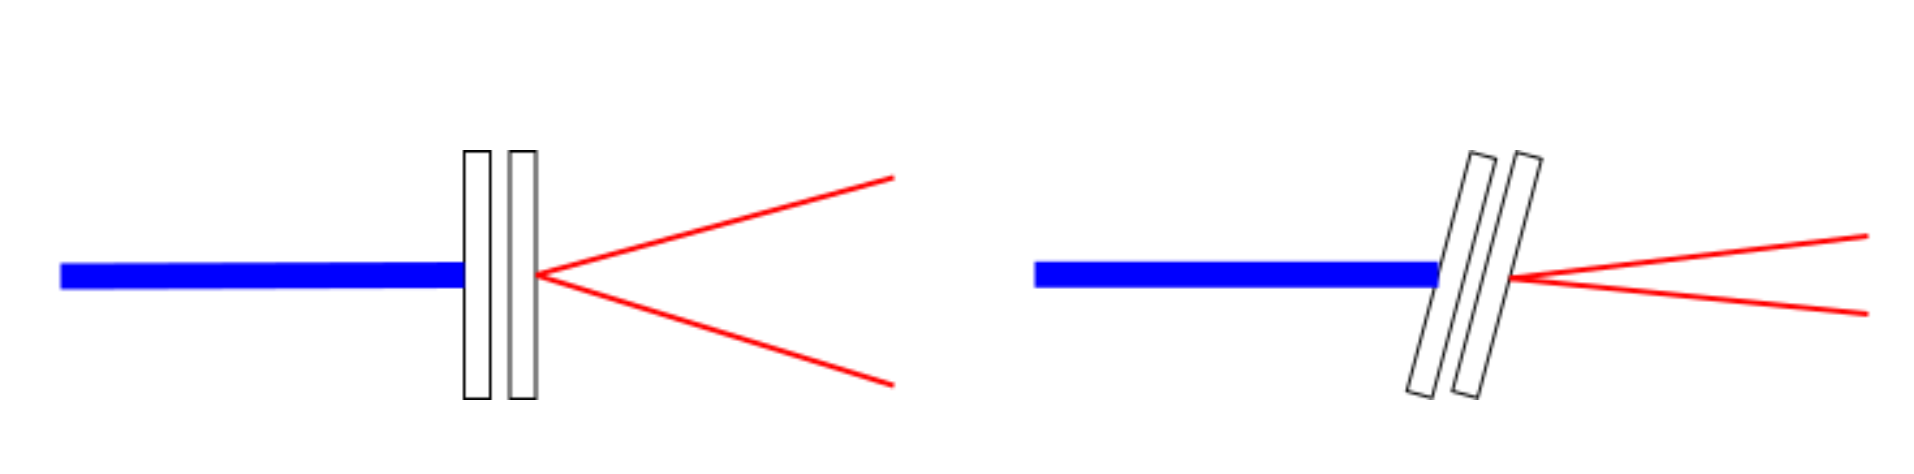
\includegraphics[width=0.5\textwidth]{Figures/Phase_matching_angle.png}
    \caption{Phase matching angle}
    \label{Phase matching angle}
\end{figure}

\subsection{Quantum output state after passing two BBO crystals}
Knowing that the pump photon is emitted with a horizontal polarization, the quantum state of the system just after the emission is - in the second quantization formalism - given by:
\begin{equation}
    |\Psi\rangle = |1_p,0_s,0_i\rangle \otimes (|H\rangle_p |-\rangle_s |-\rangle_i)
\end{equation}
where $N_p$,$N_s$ and $N_i$ are the number of photons in the pump, signal and idler modes respectively. $|H\rangle_p$ means that the pump photon is horizontally polarized. $|-\rangle_s$ and $|-\rangle_i$ are the undefined polarization states of the signal and idler photons.

The pump beam passes through a HWP (half-wave plate) that rotates the polarization of the pump photon by an angle $2\theta$, with $\theta$ being the angle of the HWP axis. The unitary operator that describes the action of the HWP on the pump photon polarization is given, in the $|H\rangle$, $|V\rangle$ basis, by:
\begin{equation}
    \hat{U}_{HWP} = \begin{pmatrix}
        \cos(2\theta) & \sin(2\theta) \\
        \sin(2\theta) & -\cos(2\theta)
    \end{pmatrix}
\end{equation}
Not here that $\hat{U}_{HWP}$ acts on the subspace of the pump photon polarization, i.e. $\hat{U}_{HWP}= \hat{U}_{HWP} \otimes \mathbb{1}_s \otimes \mathbb{1}_i$. The state of the system after the pump photon passes through the HWP is then given by:
\begin{equation}
    |\Psi\rangle' = |1_p,0_s,0_i\rangle \otimes (\cos(2\theta)|H\rangle_p + \sin(2\theta)|V\rangle_p) |-\rangle_s |-\rangle_i
\end{equation}

The beam then passes through two BBO crystals. The first BBO has an horizontal axis. This means that only horizontally polarized photons will undergo SPDC process. From the properties of the BBO crystal, the idler and signal photons will then be vertically polarized. The unitary operator that describes the SPDC process in the first BBO crystal is given by:
\begin{equation}
    \hat{U}_1 = \kappa (\hat{a}_p \hat{a}_s^\dagger \hat{a}_i^\dagger + \text{h.c.}) \otimes (|-\rangle_p|V\rangle_s|V\rangle_i \langle H|_p\langle-|_s\langle-|_i)
\end{equation}
Similarly, for the second BBO crystal, 
\begin{equation}
    \hat{U}_2 = \kappa (\hat{a}_p \hat{a}_s^\dagger \hat{a}_i^\dagger + \text{h.c.}) \otimes (|-\rangle_p|H\rangle_s |H\rangle_i \langle V|_p\langle-|_s\langle-|_i)
\end{equation}
Combining the action of both BBO crystals, the state of the system after passing through the two BBO crystals is given by:
\begin{equation}
    |\Psi\rangle'' = |0_p,1_s,1_i\rangle \otimes |-\rangle_p (\cos(2\theta)|V\rangle_s |V\rangle_i + \sin(2\theta)|H\rangle_s |H\rangle_i)
\end{equation}
Note that here the hermitian conjugate has no contribution to the state of the system. 

We recognize the entangled state for the signal and idler photons : 

\begin{equation}
    |\Phi^\theta\rangle = \cos(2\theta)|VV\rangle+ \sin(2\theta)|HH\rangle
\end{equation}
The state is said to be entangled because it is not separable, i.e. it cannot be written as a product of two states of the subsystems. It's density matrix is given by :
\begin{equation}
    \hat{\rho}_{si} = (\cos(2\theta)|VV\rangle+ \sin(2\theta)|HH\rangle)(\cos(2\theta)\langle VV|+ \sin(2\theta)\langle HH|)
\end{equation}
This state is said to be maximally entangled if $\theta = \pi/8$. In this case, the state is the Bell state $|\Phi^+\rangle = \frac{1}{\sqrt{2}}(|VV\rangle + |HH\rangle)$.

For the next subsections, the state of the system will be given in the first quantization formalism. The pump photons will be omitted as they are not relevant for the rest of the experiment. 



\subsection{Expectation values}

\paragraph{Maximally entangled state}

The signal and idler photons take two distinct paths to reach the single photon counter. They both pass through a HWP, and then a PBS (polarizing beam splitter). The PBS only transmits to the detector photons with horizontal polarization. The HWP is set at an angle $\alpha$ for the signal photon and $\beta$ for the idler photon. The operator that describes the action of the HWPs on the signal and idler photons is given by:
\begin{equation}
    \label{eq:U_HWP}
    \hat{U}_{HWP} = \hat{U}_{HWP,1} \otimes \hat{U}_{HWP,2}
\end{equation}
where
\begin{equation}
    \hat{U}_{HWP,1} = \cos(2\alpha) |H\rangle_1 \langle H|_1 + \sin(2\alpha) |V\rangle_1 \langle H|_1 + \sin(2\alpha) |H\rangle_1 \langle V|_1 - \cos(2\alpha) |V\rangle_1 \langle V|_1
\end{equation}
\begin{equation}
    \hat{U}_{HWP,2} = \cos(2\beta) |H\rangle_2 \langle H|_2 + \sin(2\beta) |V\rangle_2 \langle H|_2 + \sin(2\beta) |H\rangle_2 \langle V|_2 - \cos(2\beta) |V\rangle_2 \langle V|_2
\end{equation}
Applying this operator to $|\Phi^\theta\rangle$ gives 
\begin{equation}
    \begin{aligned}
    |\Phi^{\theta, \alpha, \beta}\rangle = &\ \cos(2\theta) \left( \sin(2\alpha)\sin(2\beta) |HH\rangle - \sin(2\alpha)\cos(2\beta) |HV\rangle \right. \\
    &\ \left. - \cos(2\alpha)\sin(2\beta) |VH\rangle + \cos(2\alpha)\cos(2\beta) |VV\rangle \right) \\
    &+ \sin(2\theta) \left( \cos(2\alpha)\cos(2\beta) |HH\rangle + \cos(2\alpha)\sin(2\beta) |HV\rangle \right. \\
    &\ \left. + \sin(2\alpha)\cos(2\beta) |VH\rangle + \sin(2\alpha)\sin(2\beta) |VV\rangle \right)
    \end{aligned}
\end{equation}

The probability of detecting both photons after they pass the PBS is the probability that both photons are in the horizontal polarization state. This probability of this is given by:
\begin{equation}
    P_{\alpha,\beta} = |\langle HH | \Phi^{\theta, \alpha, \beta}\rangle|^2 = (\cos(2\theta) \cos(2\alpha) \cos(2\beta) + \sin(2\theta) \sin(2\alpha) \sin(2\beta))^2 
\end{equation}

In this experiment, the maximally entangled state $|\Phi^+\rangle$ is chosen, i.e. setting $\theta = \pi/8 = 22.5^\circ$. The probability becomes
\begin{equation}
    P_{\alpha,\beta} = \frac{1}{2}(\cos(2\alpha) \cos(2\beta) + \sin(2\alpha) \sin(2\beta))^2 = \frac{1}{2} \cos^2(2(\alpha - \beta)) 
    \label{eq:P}
\end{equation}

\paragraph{Maximally mixed state}
Here the case where the state of the system is the maximally mixed state is considered,i.e. a non-entangled, classical state. The density matrix of the maximally mixed state is given by:
\begin{equation}
    \hat{\rho}_{si} = \frac{1}{4} \left( |HH\rangle \langle HH| + |HV\rangle \langle HV| + |VH\rangle \langle VH| + |VV\rangle \langle VV| \right)
\end{equation}
The evolve state of the system after passing through the HWPs is given by:
\begin{equation}
    \hat{\rho}'_{si} = \hat{U}_{HWP} \hat{\rho}_{si} \hat{U}_{HWP}^\dagger
\end{equation}
with $\hat{U}_{HWP}$ given by \eqref{eq:U_HWP}. 

The expectation value of the projector $\hat{\Pi}_{HH} = |HH\rangle \langle HH|$ is then given by:
\begin{equation}
    \langle \hat{\Pi}_{HH} \rangle = \text{Tr}(\hat{\rho}'_{si} \hat{\Pi}_{HH}) = \text{Tr}(\langle HH|\hat{U}_{HWP} \hat{\rho}_{si} \hat{U}_{HWP}^\dagger |HH\rangle)
\end{equation}
where the cyclic property of the trace has been used.

Then, computing term by term $ \hat{U}_{HWP} \hat{\rho}_{si}$, and keeping only the $|HH\rangle$ terms, we get:

\begin{equation}
\begin{aligned}
    \hat{U}_{HWP} |HH\rangle &= \cos(2\alpha)\cos(2\beta) |HH\rangle + \hdots \\
    \hat{U}_{HWP} |HV\rangle &=  \sin(2\alpha)\cos(2\beta) |HH\rangle + \hdots \\
    \hat{U}_{HWP} |VH\rangle &= \cos(2\alpha)\sin(2\beta) |HH\rangle + \hdots \\
    \hat{U}_{HWP} |VV\rangle &= \sin(2\alpha)\sin(2\beta) |HH\rangle+ \hdots 
\end{aligned}
\end{equation}

Then, $\hat{U}_{HWP}^\dagger = \hat{U}_{HWP}$, and 
\begin{equation}
    \text{Tr}(\langle HH|\hat{U}_{HWP} \hat{\rho}_{si} \hat{U}_{HWP}^\dagger |HH\rangle) = \frac{1}{4} \sum_{p,q = H,V} |\langle HH|\hat{U}_{HWP}|pq\rangle|^2
\end{equation}
\begin{equation}
    = \frac{1}{4} \left( \cos^2(2\alpha)\cos^2(2\beta) + \sin^2(2\alpha)\cos^2(2\beta) + \cos^2(2\alpha)\sin^2(2\beta) + \sin^2(2\alpha)\sin^2(2\beta) \right) 
\end{equation}
\begin{equation} 
    = \frac{1}{4} \left( \cos^2(2\beta)(\cos^2(2\alpha) + \sin^2(2\alpha)) + \sin^2(2\beta)(\cos^2(2\alpha) + \sin^2(2\alpha)) \right) = \frac{1}{2}
\end{equation}
So finally, 
\begin{equation}
    \langle \hat{\Pi}_{HH} \rangle = \frac{1}{2}
\end{equation}
The result hence does not depend on the angles $\alpha$ and $\beta$, which is expected for a maximally mixed state. 

\subsection{CHSH inequality}
The goal of this experiment is to violate Bell's inequality, most specifically the CHSH inequality. The CHSH inequality was derived by Clauser, Horne, Shimony and Holt in 1969. It is a generalized and most experimentally accessible form of Bell's inequality. The CSHS inequality is given by : 
\begin{equation}
    S = E(\alpha,\beta) - E(\alpha,\beta') + E(\alpha',\beta) + E(\alpha',\beta') \leq 2
    \label{CHSH}
\end{equation}
where the superior bound is given by the local hidden variable theory, and is given without proof here. In quantum mechanics, the bound can be violated by the non local correlations of entangled states. E($\alpha,\beta$) is called a correlation function, and in this experiment depend on the angles $\alpha$ and $\beta$ of the HWPs. The correlation function is given by:
\begin{equation}
    E(\alpha,\beta) = P_{HH}(\alpha,\beta) + P_{VV}(\alpha,\beta) - P_{HV}(\alpha,\beta) - P_{VH}(\alpha,\beta)
\end{equation}
where $P_{PQ}(\alpha,\beta)$ is the probability of detecting the signal and idler photons in the polarization states $P$ and $Q$ after passing through the HWPs set at angles $\alpha$ and $\beta$ respectively. It can be shown that rotating a HWP by $\pi/4$ is equivalent to measuring the opposite polarization state of the photon, e.g. $P_{HV}(\alpha,\beta) = P_{HH}(\alpha,\beta + \pi/4)$. Hence, the correlation function can be rewritten as:
\begin{equation}
    E(\alpha,\beta) = P_{\alpha,\beta} - P_{\alpha,\beta + \pi/4} - P_{\alpha+ \pi/4,\beta} + P_{\alpha+ \pi/4,\beta+ \pi/4}
\end{equation}
where $P_{\alpha,\beta}$ is the probability of detecting both maximally entangled ($\theta = \pi/8$) photons in the horizontal polarization state after passing through the HWPs set resp. at angles $\alpha$ and $\beta$. The theoretical expression of this probability is given by \eqref{eq:P}. 

The values of $\alpha$,$\beta$,$\alpha'$ and $\beta'$ are chosen such that the CHSH inequality is maximally violated. A superior bound of $2\sqrt 2$ is expected for the angles $\alpha = 0$, $\beta = \pi/16$, $\alpha' = \pi/4$ and $\beta' = 3\pi/8$. This bound is the maximal bound that can be achieved by quantum mechanics, and is called the Tsirelson bound.

The probabilities cannot be measured directly, but can be estimated by counting the number of coincidences for each of the angle pairs. The number of coincidences is the number of times the signal and idler photons are detected simultaneously by a single photon detector. One can write that $P_{\alpha,\beta} = N_{\alpha,\beta}/N_{\text{total}}$, where $N_{\alpha,\beta}$ is the number of coincidences for the angles $\alpha$ and $\beta$, and $N_{\text{total}}$ is the maximal number of coincidences that can be measured given the experimental conditions.

Finally, one can rewrite the correlation function as :
\begin{equation}
    E(\alpha,\beta) = \frac{N_{\alpha,\beta} - N_{\alpha,\beta + \pi/4} - N_{\alpha+ \pi/4,\beta} + N_{\alpha+ \pi/4,\beta+ \pi/4}}{N_{\alpha,\beta} + N_{\alpha,\beta + \pi/4} + N_{\alpha+ \pi/4,\beta} + N_{\alpha+ \pi/4,\beta+ \pi/4}}
    \label{CHSH2}
\end{equation}

The visibility is defined,
\begin{equation}
    V = \frac{N_{\text{max}} - N_{\text{min}}}{N_{\text{max}} + N_{\text{min}}}
\end{equation}
where $N_{\text{max}}$ and $N_{\text{min}}$ are the maximal and minimal number of coincidences that can be measured. The visibility is a measure of the quality of the entangled state. A visibility of 1 means that the state is maximally entangled.


\section{Experimental setup}
The experimental setup consists of a 405 nm pump beam, whose polarization is controlled by a HWP(half-wave plate). The pump beam emits horizontally polarized light and passes through a clean-up filter before reaching the BBO crystal. The beam then passes through a long-pass filter to remove residual pump light and a NPBS (non polarizing beam splitter) to separate the signal and idler beams. Each beam is then directed to a single photon detector. Additional band-pass filters are used. The single photon detector clicks when a photon reaches it, and allows to measure simultaneous detections (coincidences) of signal and idler photons, i.e. to count the number of photons created by the SPDC process. The datas are collected and analyzed by a software. It has to be noted that the path lengths of the signal and idler beams are not equal (path length difference is in the order of the cm). A delay is added in the software to compensate for this difference.

In the software, a coincidence is considered as such if two photons are detected within a given delay. In this experiment, the delay is set at $800$ps. Since the down-conversion is a highly non-probable event, only few photons are down-converted in the time scale of a photon. At this stage of the setup, with $800$ps of delay, the coincidences per second were $~250$counts/s. This means approximately one down-conversion each 4 microseconds. The $800$ps delay is hence largly acceptable.

For the second experiment, a HWP and a PBS (polarizing beam splitter) that transmits only photons with horizontal polarization are added after the NPBS for each of the signal and idler beams. 

For the third and last experiment, a second BBO crystal is added to the setup to create an entangled state. The two BBO crystals are placed side by side, but their optical axes are orthogonal. Each BBO is mounted on a rotation stage, allowing to adjust the angle of the crystal axes w.r.t. the pump beam direction of propagation. The optimal angle (phase matching angle) is the angle that maximizes the coincidences for each BBO independently, with the constraint that the optical axes of the two BBOs must be orthogonal. This last condition is verified if the number of coincidences are equal for both BBOs. To measure the coincidences for a single BBO, the polarization of the pump beam is set to horizontal and vertical in turn. 



With a delay of $800$ps, the setup before introducing the second BBO crystal and other pieces


The setup is schematically shown in Fig. \ref{fig:setup}.
\begin{figure}[H]
    \centering
    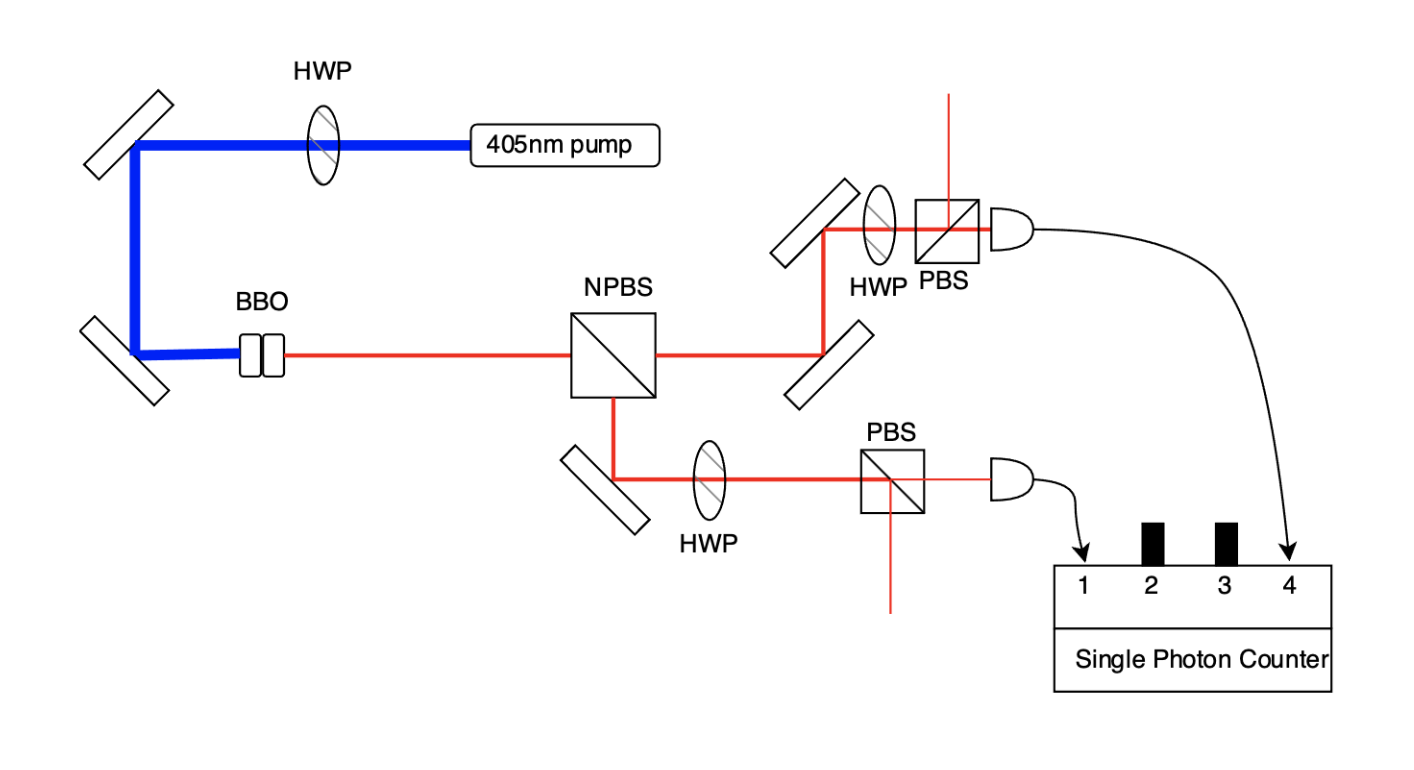
\includegraphics[width=1\textwidth]{Figures/Experimental setup.png}
    \caption{Experimental setup}
    \label{fig:setup}
\end{figure}

\section{Results and discussion}

The first step of the experiment is to mount and align the setup with one BBO crystal and without the two HWP and PBS at the end. The optical line is set up to have a clear path for the laser beam to reach the detector. Another laser is used to align the system. By putting it at both ends of the optical line, mirrors are adjusted to make the beam reach the pump. This method assures that the optical line is well aligned and the beam reaches both detectors.

The setup is very sensitive to the alignment of the mirrors and the BBO crystal and it is important to take time to align the system and verify it before starting the measurements.

\subsection{First coincidences with one BBO}

The first goal is to measure the coincidences of the photons down-converted by the BBO crystal and observe the influence of the first half wave plate (HWP), which changes the polarization of the beam, on the number of coincidences. 

The angle of the HWP is set to $0^{\circ}$ and the system is back aligned to maximize the number of coincidences. The angle of the crystal and the mirrors are adjusted.

Once the number of coincidences is stable, the angle of the HWP is changed from $(0\pm2)^{\circ}$ to $(95\pm2)^{\circ}$ by steps of $(5\pm2)^{\circ}$. For each angle, the number of coincidences is measured for 20 seconds with a binwidth of 1100 ps.

Before presenting the datas, the expected result can be calculated either in a classical frame with Jones formalism or in the quantum frame.  It will be shown below that, for this specific case, both interpretation lead to the same result. 

When a of the pump beam enters the BBO crystal, it will either collapse into the $|H\rangle$ state or in the $|V\rangle$ state, with $\cos(2\theta)$ and $\sin(2\theta)$ probabilities. If it collapses into the $|V\rangle$ state, ther is no down-conversion. If it collapses into the $|H\rangle$ state, the photon will be down-converted into two beams with $|VV\rangle$ polarization. This beam will then pass through the NPBS, which will separate the signal and idler beams. Since there is no "obstacle" between the NPBS and the detectors, the signal and idler beams will be detected simultaneously. The probability of them being detected is just given by the probability of the pump beam being in the $|H\rangle$ state, i.e. $\cos^2(2\theta)$.

Now, in a classical Frame, the Jones vector of the pump beam can be written

$$\mathbf{E_{\text{initial}}} = \begin{pmatrix} 1 \\ 0 \end{pmatrix}$$ 

Then, the Jones matrix of the HWP is given by

$$J_\text{{HWP}} = \begin{pmatrix} \cos(2\theta) & \sin(2\theta) \\ \sin(2\theta) & -\cos(2\theta) \end{pmatrix}$$ 

The BBO crystal only lets pass the horizontally polarized part of the beam and transmits two vertically polarized beams. The Jones matrix of the BBO is then

$$J_\text{{BBO}} = \begin{pmatrix} 0 & 0 \\ 1 & 0 \end{pmatrix}$$ 

Applying the Jones matrices to the pump beam, the Jones vector of the down-converted beams is 

\begin{equation}
    \mathbf{E_\text{{final}}} = J_\text{{BBO}} \cdot J_\text{{HWP}} \cdot \mathbf{E_\text{{initial}}} = \begin{pmatrix} 0 \\ \cos(2\theta) \end{pmatrix}
\end{equation}

It gives that after the combination of the HWP and the BBO crystal, the beams are vertically polarized. The intensity of the beams is the squared norm of the field 
\begin{equation}
    I(\theta) = \cos^2(2\theta)
    \label{classical malus}
\end{equation}
This is Malus' law. Since the two beams are identical, 

The results are shown in figure \ref{fig:Malus1}, and a fit is made with \eqref{classical malus} on the datas. The fit strongly suggests that the datas indeed follow Malus' law. The number of coincidences is then a good measure of the intensity of the beam. A small phase appears in the fit, which may be due to the fact that the axis of the HWP is not perfectly centered on its support. This means that when its axis is indicated to be at $0^{\circ}$, it may be slightly off. The error on the angle of the HWP, which is $2^{\circ}$, is not considered to be the cause of this phase. The distribution of the error being random around the real value of the angle, the fit would have compensated them and no phase-shift would have appeared. Another explanation could be that the incoming light is not perfectly horizontally polarized when it reaches the HWP. Hence, even with a true angle of $0^{\circ}$, the angle between the polarization of the beam and the axis of the HWP would not be $0^{\circ}$.

\begin{figure}[H]
    \centering
    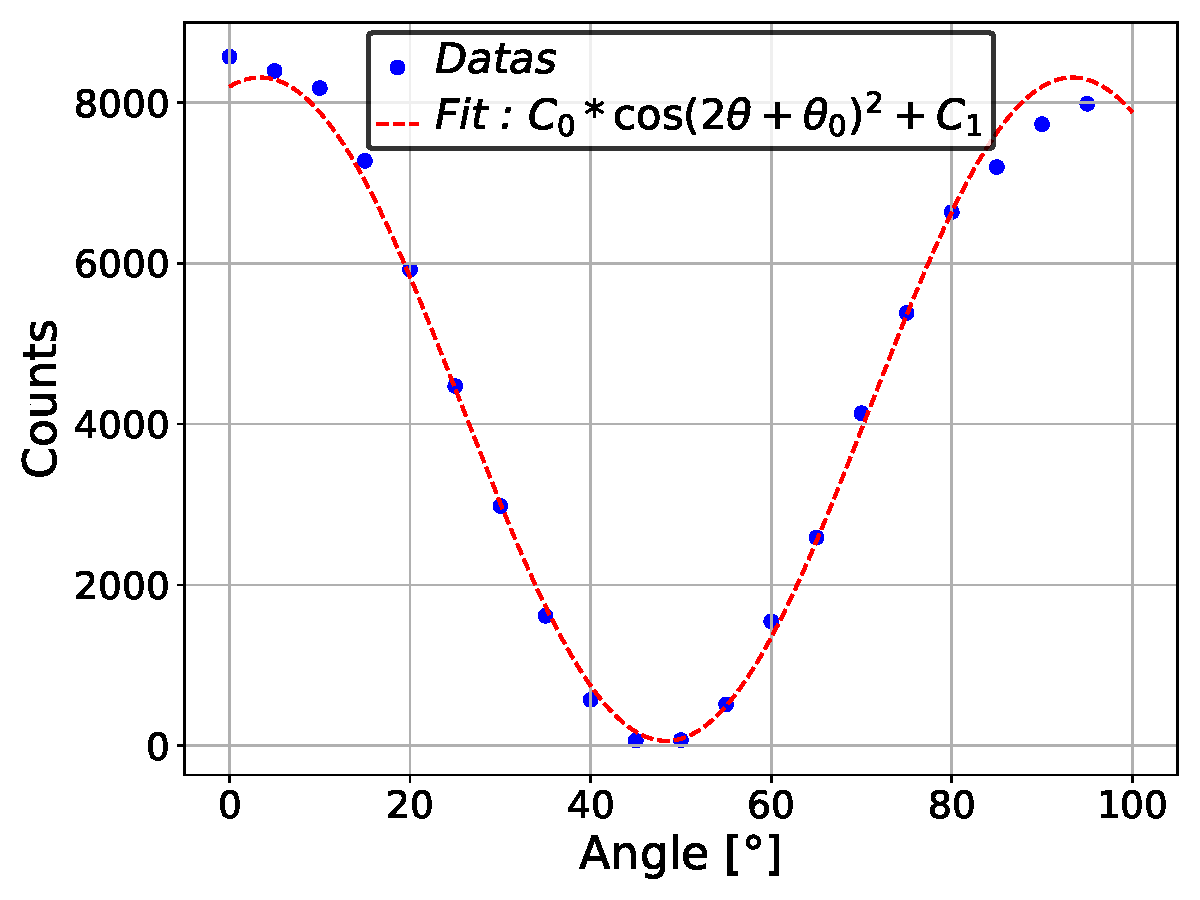
\includegraphics[width=0.7\textwidth]{Figures/Malus_HWP1.pdf}
    \caption{Number of coincidences as a function of the angle of the HWP.}
    \label{fig:Malus1}
\end{figure}

\subsection{Polarizers}

The second step is to add two HWP and two polarizing beam splitters (PBS) to the setup as shown in figure \ref{fig:setup}. The goal is to measure the coincidences of the photons emitted by the BBO crystal and observe the influence of the HWP and PBS on the number of coincidences. For this part, the HWP before the BBO crystal is removed.

The system needs to be realigned to maximize the number of coincidences because the PBS is a birefringent crystal which slightly deviates the beam.

Here, one cannot treat the system in a classical frame because the photons of the down-converted beams will collapse into a $|H\rangle$ state or a $|V\rangle$ state when passing through the HWP and PBS. The quantum formalism is then needed to describe the system and the probabilites of a coincidence to happen. 

After the BBO crystal, the state of the system is $|VV\rangle$. Both beams then pass through a HWP and a PBS. The unitary operator of the HWPs is given by \eqref{eq:U_HWP}.

The state after the two HWP is then,

\begin{align*}
    U_{HWP_1} \otimes U_{HWP_2} |VV\rangle = \sin(2\alpha) \sin(2\beta) |HH\rangle - \sin(2\alpha) \cos(2\beta) |HV\rangle \\
    - \cos(2\alpha) \sin(2\beta) |VH\rangle + \cos(2\alpha) \cos(2\beta) |VV\rangle
\end{align*}

The PBS acts as a measure on the polarization and only lets the $|HH\rangle$ photons pass. The probability of having a coincidence is then 

\begin{equation}
    P(|HH\rangle) = \left| \langle HH | U_{HWP_1} \otimes U_{HWP_2} |VV\rangle \right|^2 = \sin^2(2\alpha) \sin^2(2\beta)
    \label{P_HH}
\end{equation}

This probability is hence different from the one obtained in the first part of the experiment. It confirms that the classical frame is not adapted to describe the system. Another way to find this probability is to state that since the state is not entangled, the probability of a coincidence is the product of the probabilities of each photon to be detected in the $|H\rangle$ state.

Getting back to the measurements, both HWPs are rotated simultaneously from $(0\pm2)^{\circ}$ to $(180\pm2)^{\circ}$ by steps of $(5\pm2)^{\circ}$. For each angle, the number of coincidences is measured for 20 seconds. The results are shown in figure \ref{fig:Malus2}. The plot shows that the number of coincidences is proportional to $\sin^4(2\theta)$ (with $\alpha = \beta = \theta $) and confirms that the system follows the probability law computed in \eqref{P_HH}. 

\begin{figure}[H]
        \centering
        \includegraphics[width=0.7\textwidth]{Figures/Malus_HWP2.pdf}
        \caption{Number of coincidences as a function of the angle of the both HWP.}
        \label{fig:Malus2}
\end{figure}

Now, one HWP is set to $(45\pm2)^{\circ}$ and the other one is rotated from $(0\pm2)^{\circ}$ to $(180\pm2)^{\circ}$ by steps of $(5\pm2)^{\circ}$. For each angle, the number of coincidences is measured for 20 seconds. The results are shown in figure \ref{fig:Malus3}. The plot shows that the number of coincidences is proportional to $\sin^2(2\theta)$ and confirms that the system follows the probability law computed in \eqref{P_HH}.
    
\begin{figure}[H]
        \centering
        \includegraphics[width=0.7\textwidth]{Figures/Malus_HWP3.pdf}
        \caption{Number of coincidences as a function of the angle of the first HWP and the second fixed at $(45\pm2)^\circ$.}
        \label{fig:Malus3}
\end{figure}

For both experiments, a phase reappears in the fits. For the second experiment, the shift is of $\theta_0 = (12.8\pm0.1)^\circ$  which is not neglectable. This shift will have a crucial importance for the next experiment. The phase-shifts can be explained in the same way as for the first experiment. 

\subsection{Two BBO crystals and CSHS inequality}

The last experiment is to add a second BBO crystal to the setup perpendicular to the first one and violate the CSHS inequality. The HWP before the two crystals is set to $(22.5\pm2)^{\circ}$. Then, the state after the two crystals is the maximally entangled state $\frac{1}{\sqrt{2}}(|HH\rangle + |VV\rangle)$. Then the angle of the two HWPs after the crystals are changed with angles that are known to violate the CSHS inequality. These angles are given in the 2.5 section. For each angle, the number of coincidences is measured for 1 minute. The quantity $S$ can be calculated using \eqref{CHSH} and \eqref{CHSH2}.

The result is $S = 1.19$. The CSHS is hence not violated by the setup. A plot comparing the theoretical probabilities (given by \eqref{eq:P}) and the experimental ones is shown in figure \ref{fig:Proba}. The plot highlights the fact the experimental probabilities do not correspond to the theoretical ones.

This failure can be explained by different things. First, the visibility computed by the experimental datas is of $0.77$. Since the visibility is a measure of the quality of the entangled state, this shows that the entangled state is not perfectly prepared. The phase shift that appears in the fits of the other experiments may be the cause of this. Indeed, for the first HWP, the angle is set to $(22.5\pm2)^{\circ}$, but as it has been shown in the previous results, there could be a misalignment of the axis of the HWP w.r.t. to the support. This would lead to a slightly different angle than the one indicated, causing the entangled state to not be maximal. Then, since the angles are chosen carefully to maximize the violation of the CSHS inequality, deviation from the optimal angle can lead to a non-violation of the inequality. Further experiments taking into account the phase-shifts could be done to confirm that the HWP axis are misaligned. 

Also, the counts of coincidences for the two BBO crystals where not exactly the same, which indicates that the axis of the two BBO crystals are not perfectly orthogonal, hence leading to a non-maximal entangled state.

Clearly, the lack of time didn't allow us to perfectly align the system. It is expected that with more time, the system could be aligned better and the CSHS inequality could be violated.

\begin{figure}[H]
        \centering
        \includegraphics[width=0.7\textwidth]{TP4 Entanglement/Figures/Probabilités.pdf}
        \caption{A comparison between the theoretical probabilities and the experimental probabilities}
        \label{fig:Proba}
\end{figure}


\section{Conclusion}

In this report, the quantum entanglement phenomen has been explored and its implications for the violation of the CHSH inequality, a specific form of Bell's inequality. Experiments aimed to demonstrate the nonlocal correlations predicted by quantum mechanics using entangled photon pairs generated through spontaneous parametric down-conversion (SPDC) in a nonlinear BBO crystal.

Initially, the alignment and functionality of the experimental setup have been verified by measuring the number of coincidences with a single BBO crystal. The results confirmed the expected behavior according to Malus' law, showing that the number of coincidences varied as $\cos^2(2\theta)$ with the angle of the half-wave plate (HWP). This step was crucial for ensuring that the setup was correctly aligned and that the BBO crystal was functioning as intended.

Next, polarizing beam splitters (PBS) and additional HWPs have been introduced to further investigate the polarization states of the photons. The results were consistent with theoretical predictions, demonstrating the expected $\sin^4(2\theta)$ and $\sin^2(2\theta)$ dependencies for the number of coincidences. These experiments provided a deeper understanding of the polarization properties of the photons and the effectiveness of the setup in manipulating these states.

Finally, a second BBO crystal has been added to create an entangled state and attempted to violate the CHSH inequality. However, the measured value of $S = 1.19$ did not exceed the classical bound of 2, indicating that a violation of the CHSH inequality has not been reached. This result suggests that the entangled state was not perfectly prepared, likely due to alignment issues or imperfections in the experimental setup.

To improve the results and achieve a clear violation of the CHSH inequality, several steps can be taken. First, further refinement of the alignment process is essential to ensure that the optical paths and crystal orientations are optimized for maximum entanglement. Additionally, using higher quality optical components and more precise control of the experimental parameters could reduce noise and improve the fidelity of the entangled state.



%			Bibliographie
\begin{thebibliography}{99}

    \bibitem{Schrodinger}
    Schrödinger, E. (1935, October). Discussion of probability relations between separated systems. In Mathematical Proceedings of the Cambridge Philosophical Society (Vol. 31, No. 4, pp. 555-563). Cambridge University Press.
    
    \bibitem{EPR}
    Einstein, A., Podolsky, B., \& Rosen, N. (1935). Can quantum-mechanical description of physical reality be considered complete?. Physical review, 47(10), 777.
    
    \bibitem{Bell}
    Bell, J. S. (1964). On the einstein podolsky rosen paradox. Physics Physique Fizika, 1(3), 195.

    \bibitem{Alain Aspect}
    Aspect, A., Grangier, P., \& Roger, G. (1982). Experimental realization of Einstein-Podolsky-Rosen-Bohm Gedankenexperiment: a new violation of Bell's inequalities. Physical review letters, 49(2), 91.

    \bibitem{applications}
    Horodecki, R., Horodecki, P., Horodecki, M., \& Horodecki, K. (2009). Quantum entanglement. Reviews of modern physics, 81(2), 865-942.
    
    \bibitem{Matching-condition}
    \url{https://www.fiberoptics4sale.com/blogs/wave-optics/phase-matching-for-nonlinear-optical-processes?srsltid=AfmBOooKgcXc4ha93HrvnxejH9zEKlwWlu44McLPL41zjhsZChyu_UiP}, visited in March 2025

    \bibitem{Matching-condition2}
    \url{https://www.fiberoptics4sale.com/blogs/wave-optics/propagation-in-an-anisotropic-medium}, visited in March 2025


    
\end{thebibliography}
\end{document}
